\newpage
\section{Estabilidad de los amplificadores realimentados}
\subsection*{Introducción}
El concepto de transformación y la consecuente modificación del ancho de banda del sistema básico con función de transferencia de un solo polo, producido por la realimentación negativa se extienden al caso en que aquel tenga una función multipolo.

En efecto, sea la ganancia de lazo abierto, en Fig. \ref{fig:5.1} expresable por (\ref{eq:5.1})
\begin{figure}[H]
    \centering
    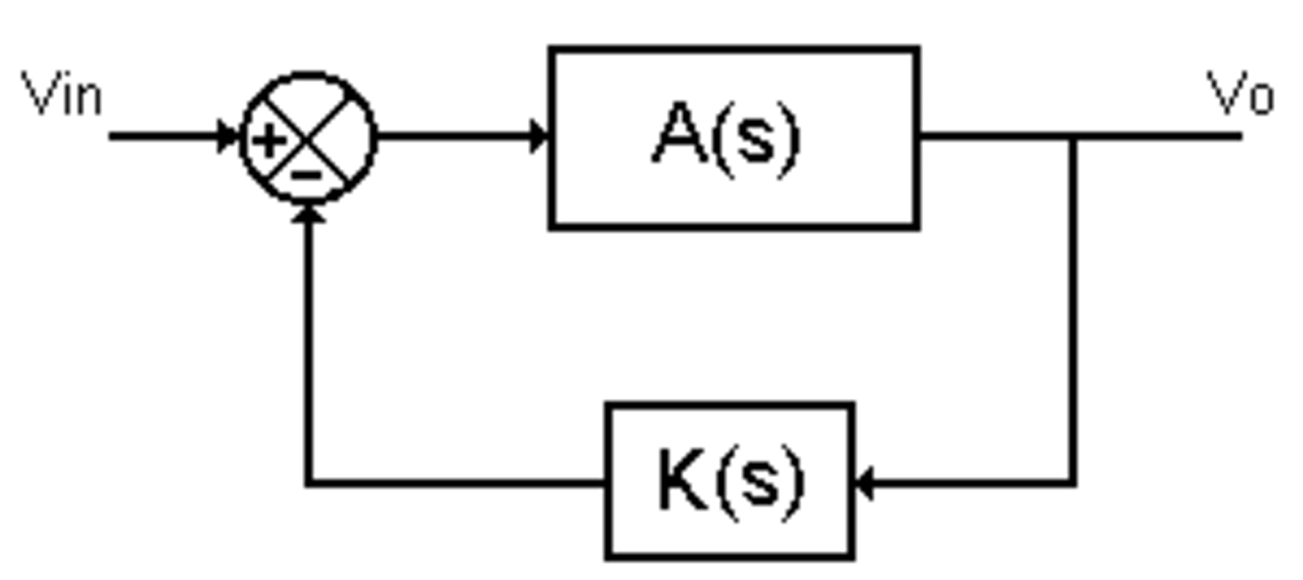
\includegraphics[width=0.5\linewidth]{Imagenes/5.1.png}
    \caption{}
    \label{fig:5.1}
\end{figure}
\begin{equation}
A_v(s) = \frac{A_v(0)}{D(s)}
\tag{5.1}
\end{equation}

En (5.1), el polinomio denominador $D(s)$, es racional a coeficientes reales en la frecuencia compleja. Si este sistema es realimentado negativamente por ejemplo con una red resistiva pura ($K=$ real), la ganancia de lazo cerrado (GLC), es

$$
A_{vf}(s) = \frac{A_v(s)}{1 - T(s)}
$$

Donde la ganancia de lazo (GL),

\begin{equation}
T(s) = -K \cdot A_v(s)
\tag{5.2}
\end{equation}

Luego se deduce para (GLC)

\begin{equation}
A_{vf}(s) = \frac{\frac{A_v(0)}{D(s)}}{1 + K \cdot \frac{A_v(0)}{D(s)}} = \left( \frac{A_v(0)}{D(s) + K \cdot A_v(0)} \right) = \frac{A'_v(0)}{D'(s)}
\tag{5.3}
\end{equation}

En la expresión (5.3), se puede ver que además de modificar la ganancia en continua también lo hace con la distribución y característica de los polos de la función de transferencia original ($A_v(s)$). Si la GLA del sistema básico tiene un solo polo (secc.2.2), la realimentación negativa introducida lo desplaza sobre el semieje real negativo (Fig. 5.2), tal que para el cien por ciento de realimentación ($K=1$), el polo adquiere una posición extrema, igual a la frecuencia de cruce de la GLA ($f_T$).
$$
f_H = K \cdot f_T \rightarrow f_H = f_T
$$
\begin{figure}[H]
    \centering
    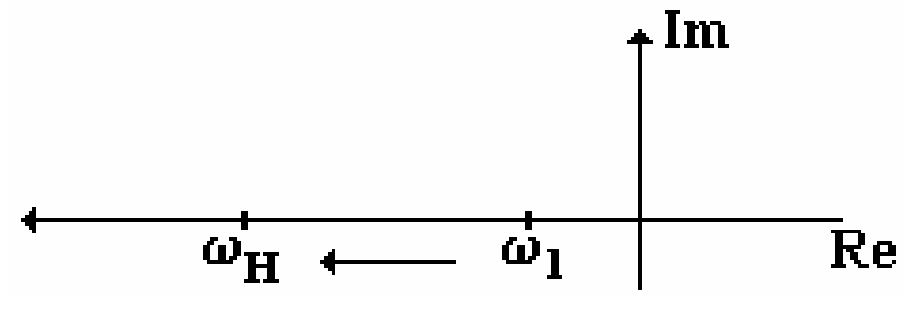
\includegraphics[width=0.5\linewidth]{Imagenes/5.2.png}
    \caption{}
    \label{fig:5.2}
\end{figure}
$\omega_1$ \quad Frecuencia del polo original de GLA. \\
$\omega_H$ \quad Frecuencia del polo de la GLC.

Se verá a continuación que si la ganancia de lazo abierto original, tiene más de un polo la introducción de realimentación negativa suficiente, puede transformar pares de estos en complejos conjugados, generando respuestas que si bien son buscadas en aplicaciones de osciladores y filtros activos, pueden ser inaceptables en amplificadores lineales de banda ancha. Para evaluar cuantitativamente estos efectos es necesario fijar algunos conceptos básicos de estabilidad de sistemas realimentados. Estos se desarrollan a partir de la expresión de la ganancia de lazo cerrado dada por la fórmula de Black, de la que matemáticamente se deduce que si en el lazo hay una señal cuya frecuencia ($\omega_G$) hace cero el denominador, el sistema se hace inestable.

En efecto si:
\begin{equation}
    1 - T(j\omega_G) = 0 \implies A_{vf}(j\omega_G) \to \infty \tag{5.4} \label{eq:5.4}
\end{equation}

La condición anterior implica un crecimiento teóricamente ilimitado de la respuesta ante la excitación de frecuencia apropiada puesta en lazo. La condición (\ref{eq:5.4}) debido a su carácter complejo, implica otras dos

\begin{equation}
    T(j\omega_G) = 1 \implies 
    \begin{cases} 
        |T(\omega_G)| = 1 & \text{(a)} \\
        Arg(T(\omega_G)) = 0 \quad \text{o} \quad 2n\pi & \text{(b)}
    \end{cases} \tag{5.5} \label{eq:5.5}
\end{equation}

Las (\ref{eq:5.5}), dan las ecuaciones de partida para la síntesis de osciladores y para el análisis de la estabilidad de amplificadores de banda ancha realimentados, donde estos últimos se deberán mantener distantes de aquella condición para operación estable. Distancias que indicaran el grado de estabilidad del amplificador y se miden tanto en módulo como en fase, denominándose márgenes. Así el margen de ganancia (MG), indica cuan diferente de uno es el módulo a la frecuencia que satisface la condición de fase (\ref{eq:5.5}b) y viceversa el margen de fase (M$\varphi$), muestra la diferencia de la fase actual y la que satisfaría la condición (\ref{eq:5.5}a) es decir, cuando el módulo de la ganancia de lazo es unitario. \\
Fig \ref{fig:5.3}.
\begin{figure}[H]
    \centering
    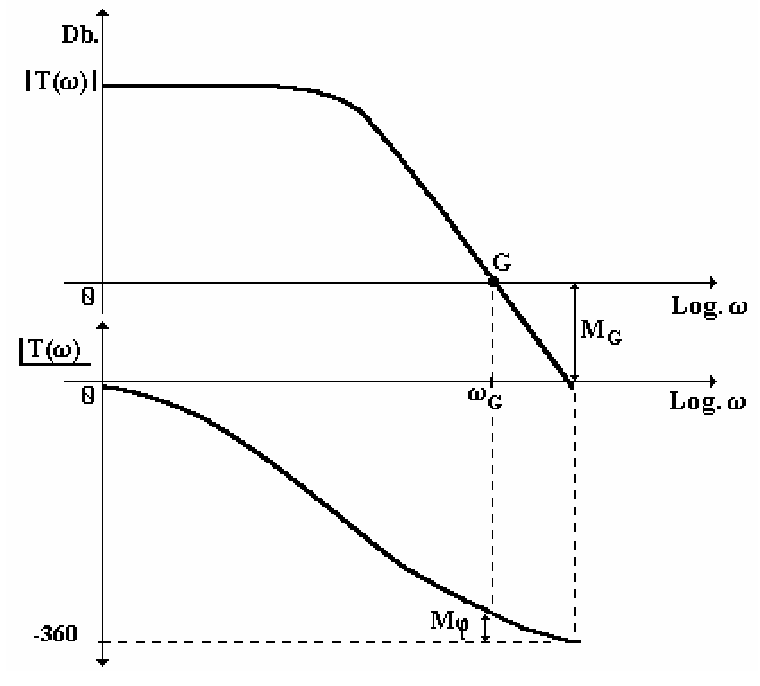
\includegraphics[width=0.5\linewidth]{Imagenes/5.3.png}
    \caption{}
    \label{fig:5.3}
\end{figure}
Existen varios criterios o métodos para evaluar el grado de estabilidad de un sistema ( Nyquist; Mikailov, Bode, etc.). En este texto se utilizaran los diagramas de Bode por su simplicidad.

No obstante cualquiera de los márgenes definidos permiten medir el grado de estabilidad de un sistema, es más utilizado el de fase, debido a que en un amplificador estable la condición de módulo (\ref{eq:5.5}a), se satisface siempre a una frecuencia más baja que la (\ref{eq:5.5}b), tal como lo muestra Fig \ref{fig:5.3}.
Para evaluar cuantitativamente este último y a los efectos de generalizar, se considerará que la red de realimentación es función de la frecuencia ($K(s)$). Luego la ganancia de lazo es según (5.2).

\begin{equation}
    T(s) = -K(s).A_v(s) \tag{5.6} \label{eq:5.6}
\end{equation}

La condición de fase planteada a la frecuencia del punto crítico ($\omega_G$), será teniendo en cuenta que la realimentación negativa introduce un atraso de $180^\circ$, como lo indica la siguiente:

\begin{equation*}
    \angle T(\omega_G) = \angle -1 + \angle K(\omega_G) + \angle A_v(\omega_G) = -180 + \angle K(\omega_G).A_v(\omega_G)
\end{equation*}

\begin{equation}
    M_\Phi = -180^\circ + Arg( K(\omega_G).A_v(\omega_G) ) + 360^\circ = Arg( T(\omega_G) ) + 180^\circ \tag{5.7} \label{eq:5.7}
\end{equation}

En un sistema estable el atraso de fase producido por la ganancia de lazo deberá ser menor de $180^\circ$ y en consecuencia el margen resultará un número positivo.

La frecuencia del punto crítico ($\omega_G$) se evalúa a partir de la condición de módulo

\begin{equation}
    |T(\omega_G)| = 1 \implies \left| A_v(\omega_G) \right| = \left| \frac{1}{K(\omega_G)} \right| \tag{5.8} \label{eq:5.8}
\end{equation}

En este punto es necesario aclarar el sentido que toman los términos involucrados en la expresión de la ganancia de lazo cuando es utilizada en el análisis de estabilidad del amplificador. En primer lugar hay que tener presente que aquella se define como la tendría una señal intercalada en el, cuando la señal que se debe amplificar está pasivada, en este caso particular la señal a insertar en el lazo es el ruido eléctrico siempre presente y cuyo espectro infinito puede aportar la componente que satisfaga las expresiones (\ref{eq:5.5}). El componente de ruido dominante en la mayoría de las aplicaciones es la tensión de ruido interno del amplificador ($v_n$), que por conveniencia es reducido a un modo diferencial equivalente en serie con la entrada  no inversora de aquel (\ref{eq:5.4}), de la misma manera que se hace con la tensión de Offset y RRMC para manifestar su efecto. 
\begin{figure}[H]
    \centering
    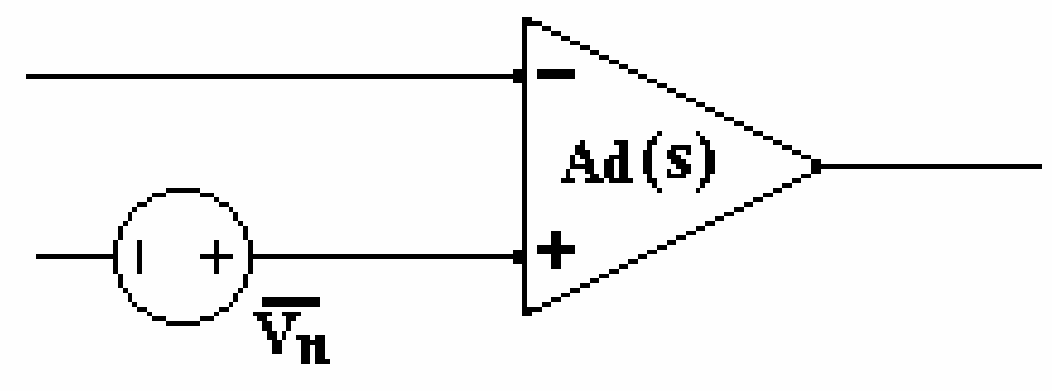
\includegraphics[width=0.5\linewidth]{Imagenes/5.4.png}
    \caption{}
    \label{fig:5.4}
\end{figure}

En base a lo expuesto se puede argumentar que el análisis de estabilidad de una aplicación amplificadora cualquiera, es equivalente a hacerlo con esta excitada por el generador de ruido como muestra la fig \ref{fig:5.4}, luego, la ganancia de lazo de este amplificador resulta, según lo analizado en (1.2), en la siguiente

\begin{equation*}
    T(s) = -K(s).A_d(s)
\end{equation*}

Finalmente, interpretando (\ref{eq:5.8}) en estos términos se obtiene (5.9)

\begin{equation}
    |T(\omega_G)| = 1 \implies |A_d(\omega_G)| = \left| \frac{1}{K(\omega_G)} \right| \tag{5.9} \label{eq:5.9}
\end{equation}

En esta última se distingue que, el primer término se corresponde con la ganancia de lazo abierto del amplificador en configuración no inversora, que además es la que tendría el generador de ruido de fig \ref{fig:5.4}, razón por la cual a la función de transferencia del amplificador básico ($Ad(s)$), se la denomina \textit{ganancia de lazo abierto de ruido}, ( $Ad=GLAn$), mientras que el segundo termino es la ganancia no inversora ideal del mismo amplificador, motivo por el cual se la llama también \textit{ganancia de lazo cerrado de ruido}, ($Avfin = 1/K$). A lo largo de este texto se utilizarán indistintamente la simbología dada por (\ref{eq:5.9}) o sus equivalentes arriba definidas.

A partir de (\ref{eq:5.5}) se deduce que el punto crítico (G) se encuentra en la intersección del diagrama de módulo de la $GLAn$ y $Avfin=1/K(s)$ como muestra las fig \ref{fig:5.5}, en la que se ha supuesto una aplicación que utiliza un A.O con ganancia de modo diferencial de un solo polo y red de realimentación resistiva pura ($K=real$).

\begin{gather*}
    A_d(s) = \frac{A_d(o)}{1 + \frac{s}{\omega_1}} \\
    GLAn = A_v(\omega) = A_d(\omega)
\end{gather*}
\begin{figure}[H]
    \centering
    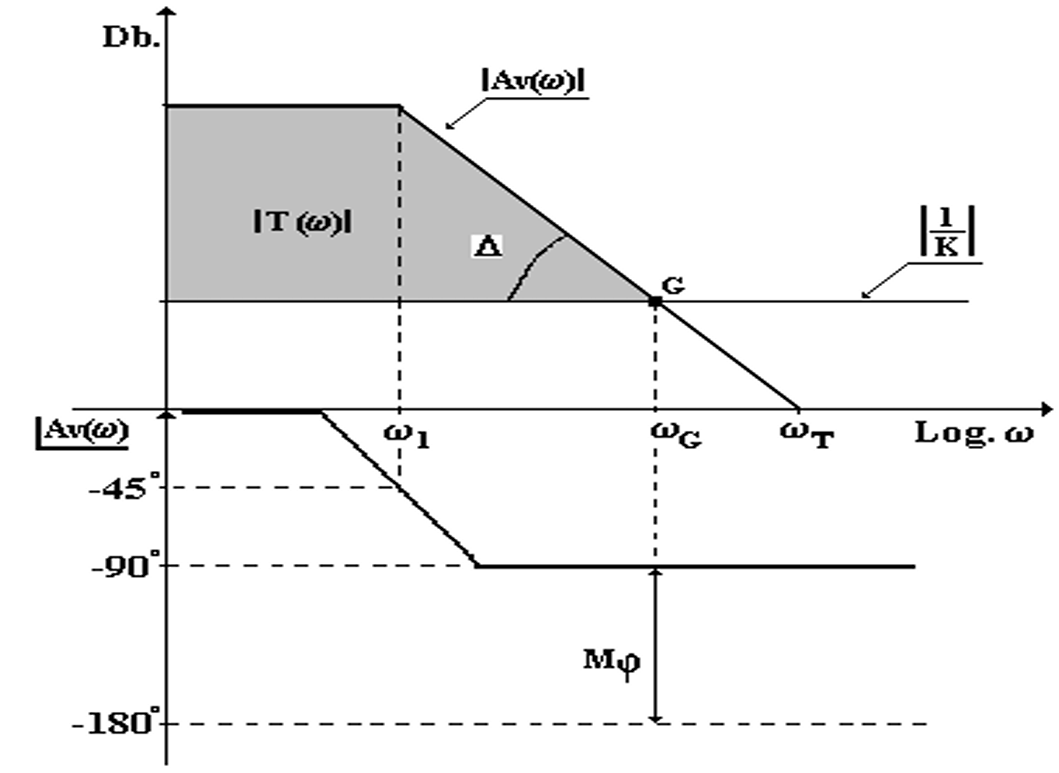
\includegraphics[width=0.5\linewidth]{Imagenes/5.5.png}
    \caption{}
    \label{fig:5.5}
\end{figure}

Del diagrama asintótico se deduce para el margen de fase el siguiente valor

\begin{equation*}
    M_{\Phi} = Arg( T(\omega_G) ) + 180^\circ = Arg( A_v(\omega_G) ) + 180^\circ = 90^\circ
\end{equation*}

Una manera cualitativa de evaluar la estabilidad del sistema es mediante un indicador que es fácilmente identificable en el diagrama de módulos de las magnitudes involucradas y es la pendiente relativa ($\Delta$ )entre la ganancia de lazo abierto y la de ruido ($1/K$) en el punto crítico (G) o de cierre, del diagrama de módulo de T. Si dicha pendiente es menor que - 40 dB/ dec, indicaría cierto grado de estabilidad, tal es el caso planteado en Fig.\ref{fig:5.5} donde $\Delta = - 20 dB/dec$ y el margen de fase igual a $+90^\circ$, mientras que el diagrama de Fig.\ref{fig:5.6}, indicaría inestabilidad, ( $\Delta = -60 dB/dec \Rightarrow M_\phi < 0^\circ$ ).
\begin{figure}[H]
    \centering
    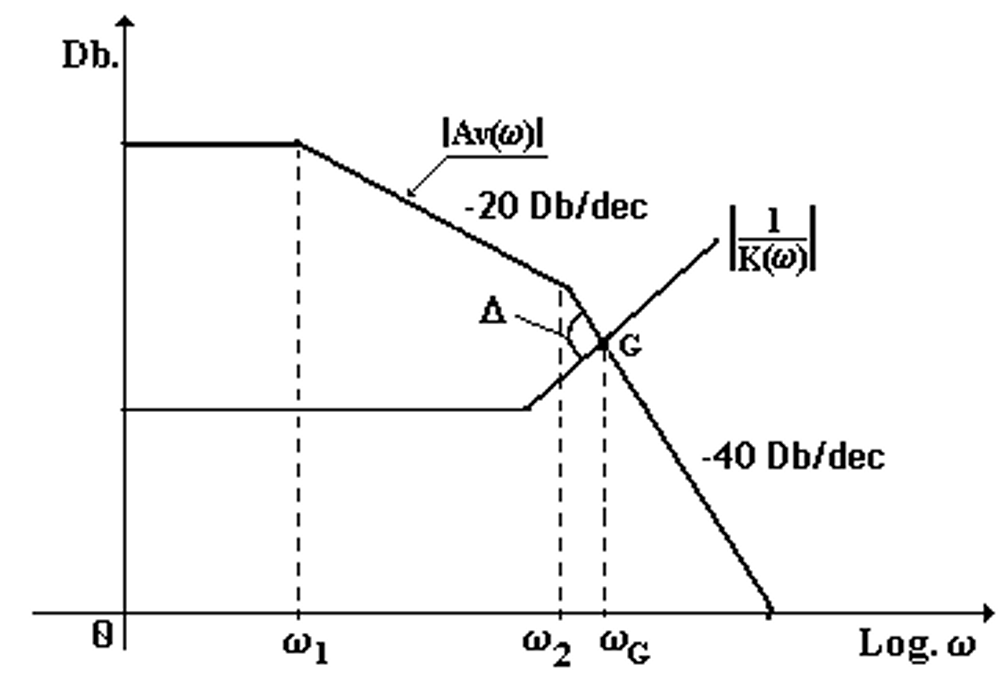
\includegraphics[width=0.5\linewidth]{Imagenes/5.6.png}
    \caption{}
    \label{fig:5.6}
\end{figure}

\subsection{Sistema con Ganancia de Lazo de Dos Polos}
Un sistema con ganancia de lazo de dos polos, puede llegar a tener un comportamiento dinámico inaceptable para operar como amplificador, según sea la cantidad de realimentación introducida.

En efecto si:

\begin{equation}
    T(s) = -K(s).A_d(s) = \frac{-To}{\left(1 + \frac{s}{\omega_1}\right).\left(1 + \frac{s}{\omega_2}\right)} \tag{5.10} \label{eq:5.10}
\end{equation}

El margen de fase será :

\begin{equation}
    M\phi = -\left( \text{tg}^{-1}\left(\frac{\omega_G}{\omega_1}\right) + \text{tg}^{-1}\left(\frac{\omega_G}{\omega_2}\right) \right) + 180^\circ \tag{5.11} \label{eq:5.11}
\end{equation}
\[ \omega_G \to \infty \quad \Rightarrow \quad M\phi \to 0^\circ \]

Se puede analizar el comportamiento dinámico de un amplificador de estas características a partir de la expresión genérica de la GLC dada por (2.12). En efecto normalizando esta en amplitud y relacionándola con T(s) dada por (\ref{eq:5.10}), se obtiene

\begin{gather*}
    A_{vf}(s) = \frac{A_{vfi}}{\left( 1 - \frac{1}{T(s)} \right)} \Rightarrow a_{vf}(s) = \frac{1}{\left( 1 - \frac{1}{T(s)} \right)} \\
    a_{vf}(s) = \frac{1}{\left( 1 + \left( 1 + \frac{s}{\omega_1} \right).\left( 1 + \frac{s}{\omega_2} \right) . \frac{1}{T_0} \right)}
\end{gather*}

\begin{equation}
    avf_{(s)} \cong \frac{1}{\left( 1 + \frac{s}{(T_0)}\left(\frac{1}{\omega_1} + \frac{1}{\omega_2}\right) + \frac{s^2}{(T_0).\omega_1.\omega_2} \right)} \tag{5.12} \label{eq:5.12}
\end{equation}

El denominador de (\ref{eq:5.12}) tiene la forma clásica de respuesta de los sistemas de 2do. orden, cuya expresión compacta parametrizada es

\begin{equation}
    a_{vf}(s) = \frac{1}{1 + \frac{s}{\omega_P.Q_P} + \frac{s^2}{\omega_P^2}} \tag{5.13} \label{eq:5.13}
\end{equation}

$\omega_P =$ frecuencia del polo \\
$Q_P =$ factor de calidad a la frecuencia del polo
Las equivalencias entre los coeficientes es de (\ref{eq:5.12}) y (\ref{eq:5.13}) son

\begin{equation}
    \omega_P = \sqrt{T_0.\omega_1.\omega_2} \quad \text{y} \quad Q_P = \frac{T_0}{\omega_P} \left( \frac{\omega_1.\omega_2}{\omega_1 + \omega_2} \right) \tag{5.14} \label{eq:5.14}
\end{equation}

A los efectos de simplificar el análisis de la respuesta de la ganancia de lazo cerrado conviene normalizar en frecuencia la expresión (\ref{eq:5.13}) respecto de la frecuencia $\omega_P$.

\begin{equation*}
    \frac{s}{\omega_P} = \frac{j\omega}{\omega_P} = J\Omega = S
\end{equation*}

Luego la (\ref{eq:5.13}) queda:

\begin{equation}
    a_{vf}(s) = \frac{1}{1 + \frac{S}{Q_P} + S^2} \tag{5.15} \label{eq:5.15}
\end{equation}

Las caracteristicas de los polos de la expresión (\ref{eq:5.15}) definirán las respectivas de la respuesta de lazo cerrado del sistema, en términos del Qp.

\begin{equation*}
    S_{1}; S_{2} = \frac{1}{2} \left( \frac{-1}{Q_P} \pm \sqrt{\frac{1}{Q_P^2} - 4} \right)
\end{equation*}

En efecto de la anterior, se deduce que $Q_P = 0,5$ da el caso crítico (raíces reales iguales) siendo complejas conjugadas para factores de calidad mayores y reales distintas en caso contrario.

El efecto que tiene la cantidad de realimentación (K), sobre la mutación polar se ve en Fig.\ref{fig:5.7}.

Definiendo la relación, (o distancia en escala logarítmica), de frecuencia entre los polos de la ganancia de lazo (\ref{eq:5.10})

\begin{equation*}
    D_P = \frac{\omega_2}{\omega_1}
\end{equation*}

Se puede expresar (\ref{eq:5.14}) como:

\begin{equation}
    Q_P = \frac{\sqrt{T_0.D_P}}{D_P + 1} \cong \sqrt{\frac{T_0}{D_P}} = \sqrt{\frac{K.A_v(0)}{D_P}} \tag{5.16} \label{eq:5.16}
\end{equation}
La (\ref{eq:5.16}) muestra que definida la respuesta a lazo abierto del sistema, la característica de los polos estará determinada exclusivamente por la cantidad de realimentación introducida, tal que para

\begin{align*}
    Q_P = 0.5 &\implies K_{crit} \implies RRI \\
    Q_P > 0.5 &\implies K > K_{crit} \implies RCC \\
    Q_P < 0.5 &\implies K < K_{crit} \implies RRD
\end{align*}

La figura \ref{fig:5.7a}, muestra lo comentado en el plano complejo y la \ref{fig:5.7b} lo hace en módulo y fase de la ganancia de lazo respectivo
\begin{figure}[H]
    \centering
    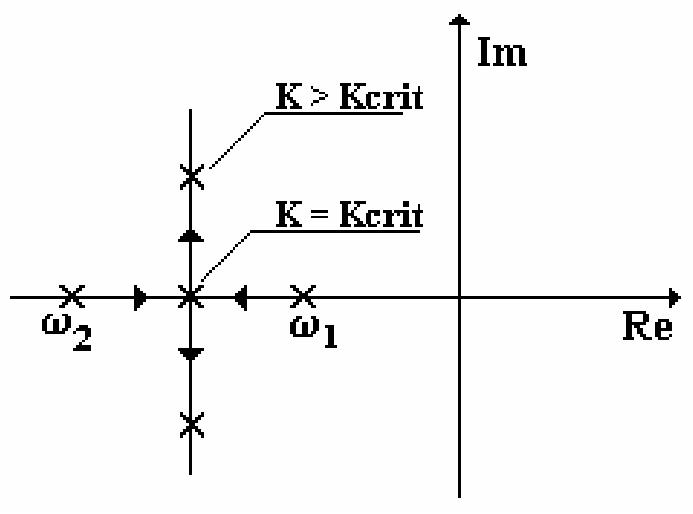
\includegraphics[width=0.5\linewidth]{Imagenes/5.7a.png}
    \caption{}
    \label{fig:5.7a}
\end{figure}

\begin{figure}[H]
    \centering
    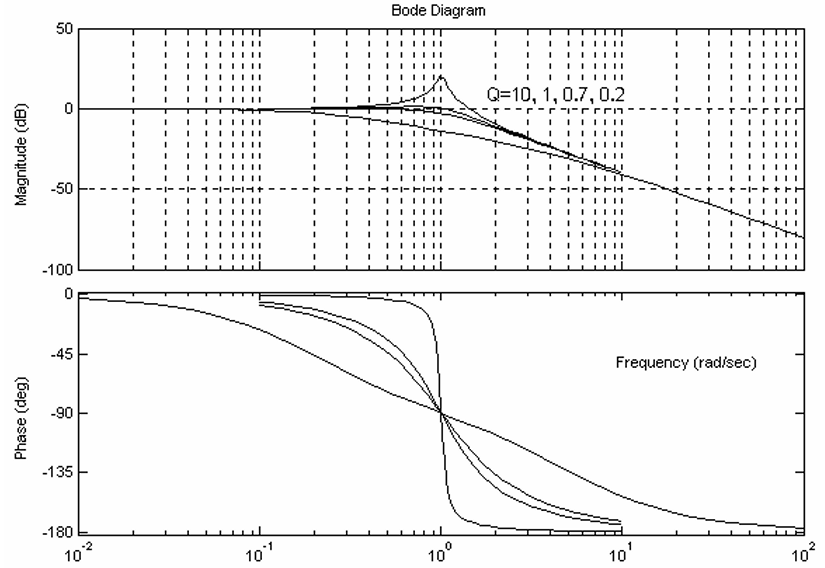
\includegraphics[width=0.5\linewidth]{Imagenes/5.7b.png}
    \caption{}
    \label{fig:5.7b}
\end{figure}
Obviamente el efecto, sobre la respuesta, del tipo de raíces, es sustantivo. Se puede ver que según crece el valor de Qp, la respuesta se aproxima a la producida por un circuito resonante (RLC), casos estos inaceptables en amplificación lineal. Desde este punto de vista aquello debe ser interpretado como un deterioro del grado de estabilidad del sistema. Esto se puede cuantificar midiendo el margen de fase. La fig \ref{fig:5.8} muestra un caso particular en que la frecuencia del punto crítico coincide con el segundo polo de la ganancia de lazo abierto ( $\omega_G = \omega_2$ y $\omega_2 \gg \omega_1$ ). El margen de fase resultante en este caso es

\[
    M\varphi = \left| \underline{K.A_v(\omega_G)} \right. + 180 = - \left( \text{tg}^{-1} \frac{\omega_G}{\omega_1} + \text{tg}^{-1} \frac{\omega_G}{\omega_2} \right) + 180 \cong 45^\circ
\]
En la medida que $\omega_G$ sea mayor que $\omega_2$, disminuye el grado de estabilidad del amplificador.

El factor de calidad (Qp), involucrado se deduce fácilmente teniendo en cuenta el carácter logarítmico del diagrama de módulos de fig 5.8.

\begin{equation*}
    \frac{20 \left( \log A_d(0) - \log \left( \frac{1}{k} \right) \right)}{(\log \omega_2 - \log \omega_1)} = 20 \frac{dB}{dec} \quad \Rightarrow \quad A_d(0).k = \frac{\omega_2}{\omega_1} = D_p
\end{equation*}

Luego de (\ref{eq:5.16}) se deduce Qp=1
\begin{figure}[H]
    \centering
    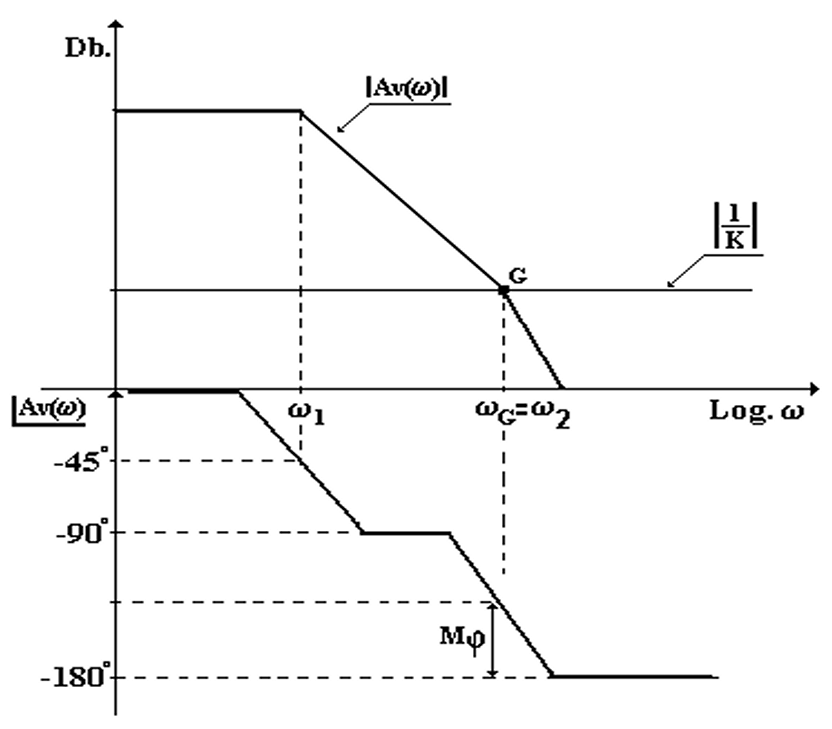
\includegraphics[width=0.5\linewidth]{Imagenes/5.9.png}
    \caption{}
    \label{fig:5.9}
\end{figure}
A la luz del análisis expuesto se entiende el problema de estabilidad que pueden presentar los amplificadores realimentados activamente, aún en el caso que utilicen amplificadores internamente compensados, como es el ejemplo del amplificador logarítmico analizado en la sección 2.2 (E.2.3), cuya estabilidad se analiza en el ejemplo siguiente.
\noindent\rule{\textwidth}{1pt} % Línea 
\textbf{\large Ejemplo 5.1}\\
\noindent\rule{\textwidth}{1pt} % Línea 
\vspace{0.5cm}

Calcular el margen de fase del ampli-log, del ejemplo E 2.3, si el VFA OPA627 utilizado presenta un segundo polo en $f_2 = 50 \text{ MHz}$. \\
El análisis siguiente toma como referencia inicial las figuras y valores de las magnitudes relevantes calculadas en E 2.3.

\vspace{0.2cm}
horizontal
\vspace{0.2cm}

Los datos aplicables del amplificador utilizado son,

\vspace{0.3cm}

OPA 627: \quad $A_d(0)= 116 \text{ dB} \quad f_1= 25 \text{ Hz} \quad f_T= 16 \text{ MHz} \quad f_2= 50 \text{ MHz}$
Teniendo presente que la ganancia de lazo, dependiente de la amplitud de señal resultaba para su valor máximo, ($v_{imax} = 10\text{V} \Rightarrow T_0 = 168 \text{ dB}$ ) y nominando como $A'_d(0)$ a la distancia en dB que hay desde el origen hasta la ordenada correspondiente a la frecuencia $f_2$ , se deduce de la figura E 2.3.2, el margen de fase respectivo.

Teniendo presente el carácter logarítmico del diagrama

$A'_d(0) = f_2 / f_T = 3.13 \implies 9.9 \text{ db} \implies (A_d(0)) = + A'_d(0))_{\text{dB}} \cong 126 \text{ db} = \mathbf{(A)}_{\text{db}}$

$((T_0)_{\text{dB}} - \mathbf{(A)}_{\text{dB}}) / \log(f_G / f_2) = 40 \text{ db/dec} \implies f_G = f_2 \sqrt{(T_0/A)} \cong 561 \text{MHz}$

Con valor de la frecuencia del punto crítico calculada, resulta un margen de fase de $\Phi_M \cong 5^\circ$

Lo reducido de este último resultado se agravaría al punto de llevarlo a oscilación ($\Phi_M = 0^\circ$), si se tienen en cuenta el atraso de fase adicional que producen las capacidades parásitas asociadas a los terminales de entrada del amplificador, (Caso que será tratado posteriormente).
Una manera de mejorar el margen de fase es, disminuyendo la dependencia directa que tiene la ganancia de lazo con señal aplicada, esto es atenuando la cantidad de realimentación $K_0$. Esto se logra por atenuación de la señal a realimentar, con el agregado de una resistencia en serie con el emisor del transistor.
En efecto recalcando la cantidad de realimentación con el agregado de $R_e$ en serie con $h_{ib}$, en el modelo reducido de figura E 2.3.1, se obtiene

\begin{equation*}
    K|_{v_{in}=0} = \frac{V^-}{V'} = g_m . R_1 . \left( \frac{h_{ib}}{h_{ib} + R_e} \right)
\end{equation*}

La anterior muestra la atenuación introducida por $R_e$, que se traslada a la ganancia de lazo.

\begin{equation*}
    T_0 = -I_C . R_1 . \left( \frac{h_{ib}}{h_{ib} + R_e} \right) . \frac{A_d(0)}{V_t} = \left( \frac{V_{in}}{V_t} \right) . \left( \frac{h_{ib}}{h_{ib} + R_e} \right) . A_d(0)
\end{equation*}

La anterior muestra que la resistencia de emisor limitaría el valor de la ganancia de lazo para valores elevados de corriente de colector ($h_{ibmin} = V_t / I_{Cmax}$) y aunque desde este punto de vista convendría que $R_e$ fuera lo más elevado posible, sería a costas de la excursión de la tensión de salida, debido a esto en aplicaciones típicas del amplificador logarítmico, su valor no supera los $5 \text{ k}\Omega$. Asumiendo $R_e = 2 \text{ k}\Omega$, se obtiene para señal de entrada máxima.

$h_{ibmin} = 250 \text{ Ohms}$

$T_0 = 168 \text{ dB} - 20 \text{ dB} = 148 \text{ dB}$

$f_G = f_2 \sqrt{(T_0/A)} = 177 \text{ Mhz} \implies \Phi_M \cong 16^\circ$

Esta mejora relativa del margen de fase es todavía insuficiente para tener una respuesta dinámica aceptable.
Otra manera de analizar la estabilidad del sistema es a través de la respuesta en el dominio temporal, a un escalón de tensión unitaria U(t). Aplicando la transformada inversa de Laplace a la ganancia de lazo cerrado normalizada en amplitud

\begin{equation}
    v_{on}(t) = \mathcal{L}^{-1} [ ( U(s) . a_{vf}(s) ) ] = \mathcal{L}^{-1} \left[ \frac{1}{s} \cdot \frac{1}{D(s)} \right] \tag{5.17} \label{eq:5.17}
\end{equation}

En el caso en que el polinomio denominador tenga raíces reales distintas (caso sobre amortiguado),

\begin{equation*}
    \frac{1}{D(s)} = \frac{1}{(s + a_1)(s + a_2)}
\end{equation*}

La respuesta temporal tendrá únicamente componentes exponenciales decrecientes.

\begin{equation}
    v_{on}(t) = 1 - B \left( \frac{1}{A_1} e^{-a_1 \cdot t} - \frac{1}{A_2} e^{-a_2 \cdot t} \right) \tag{5.18} \label{eq:5.18}
\end{equation}

En cambio si las raíces son complejas conjugadas (caso subamortiguado) aparecen componentes senoidales amortiguadas exponencialmente

\begin{equation}
    v_{on}(t) = 1 - e^{-A \cdot t} ( B_1 \cdot Sen(c \cdot t) + Cos(c \cdot t) ) \tag{5.19} \label{eq:5.19}
\end{equation}

La Fig. 5.9 muestra la respuesta normalizada a un escalón unitario para distintos valores de Qp.

El efecto sensible producido por el aumento de la cantidad de realimentación es el de disminuir el tiempo de crecimiento (tiempo de respuesta) pero a expensas de aumentar la amplitud de los componentes senoidales (rebase o peaking). En la Fig. 5.10 se detallan los parámetros característicos contenidos y definidos a partir de la forma de onda de la respuesta.
\begin{figure}[H]
    \centering
    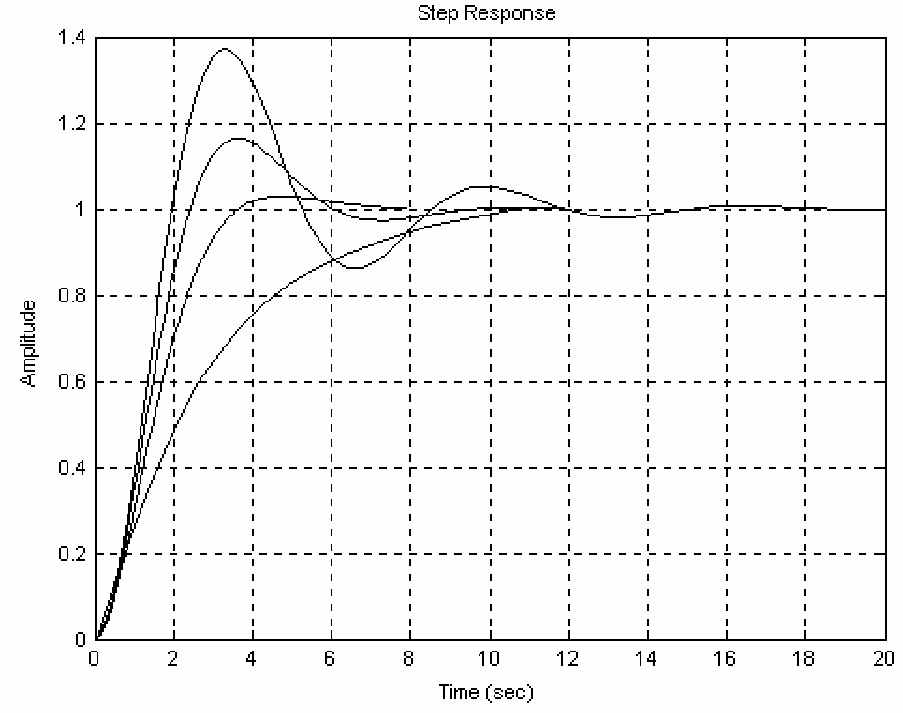
\includegraphics[width=0.5\linewidth]{Imagenes/5.10.png}
    \caption{}
    \label{fig:5.10}
\end{figure}
\begin{figure}[H]
    \centering
    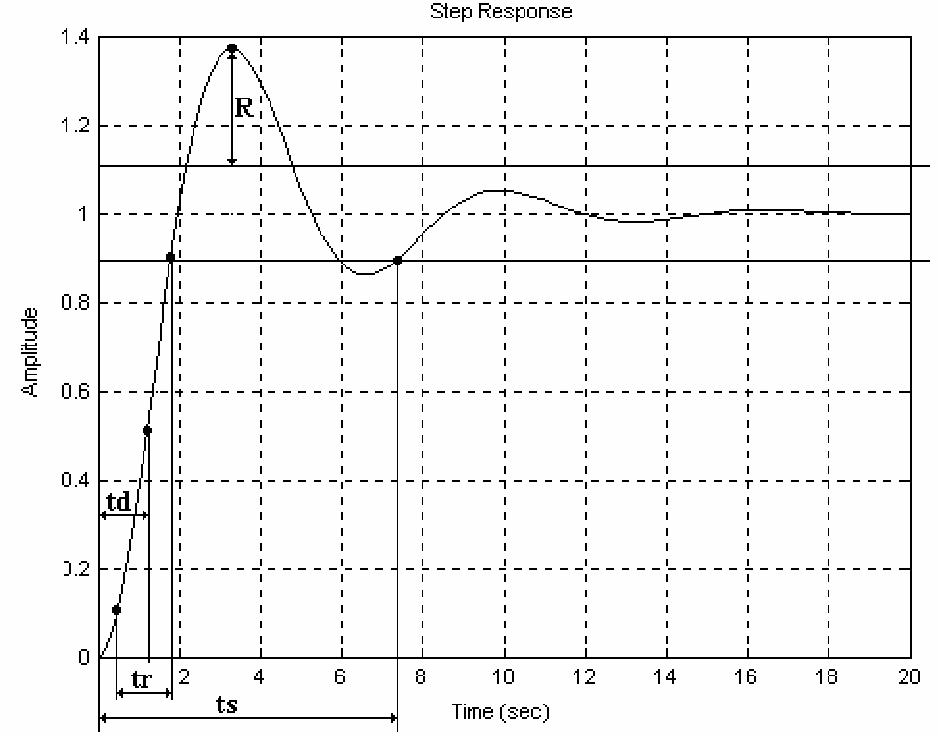
\includegraphics[width=0.5\linewidth]{Imagenes/5.11.png}
    \caption{}
    \label{fig:5.11}
\end{figure}
\begin{itemize}
    \item $t_s =$ tiempo de establecimiento
    \item $t_r =$ tiempo de crecimiento
    \item $t_d =$ tiempo de retardo
    \item $Rebase =$ pico máximo de la respuesta respecto del valor de estado estacionario.
\end{itemize}

En el caso de un amplificador con tres polos reales en lazo abierto se demuestra que, el aumento de la cantidad de realimentación negativa introducida produce reducción del margen de fase que puede hacerse negativo (Inestabilidad).
\subsubsection{Análisis de Estabilidad del CFA}
Si bien los conceptos de estabilidad desarrollados tienen validez general, el caso de los CFA merece un análisis adicional. En efecto el modelo de un solo polo asumido para la transimpedancia dado por (3.1) es suficientemente preciso, para evaluar efectos de primer orden en el comportamiento del dispositivo como lo muestran las expresiones deducidas allí. No obstante, no es difícil intuir que la presencia de componentes capacitivos parásitos asociados a las impedancias de entrada y salida, necesariamente han de agregar otros polos a la transimpedancia y las expresiones con ellas derivadas.

Esto se puede apreciar claramente en los gráficos de magnitud y fase de transimpedancia publicados en la hoja de datos de un dispositivo comercial (OPA 603-BB), mostrado en fig.5.11, en la que se observa un crecimiento abrupto del atraso de fase a frecuencias superiores a los 100 MHz, indicando la presencia de otro polo en las cercanías, en consecuencia debido a que la transimpedancia participa en la expresión de la ganancia de lazo (3.3), es de esperar que en determinadas condiciones de operación se produzca inestabilidad.

Efectuando un análisis cuantitativo del problema a partir de la ganancia de lazo (3.3) expresada a la frecuencia del punto crítico, se obtiene la siguiente relación.

\begin{equation}
    |T(\omega_G)| = 1 = \frac{|Z_T(\omega_G)|}{R_2} \implies R_2 = |Z_T(\omega_G)| \tag{5.20} \label{eq:5.20}
\end{equation}

El margen de fase resulta

\begin{equation}
    \varphi_m = \angle T(\omega_G) + 180^\circ = \angle Z_T(\omega_G) + 180^\circ \tag{5.21} \label{eq:5.21}
\end{equation}


\begin{figure}[H]
    \centering
    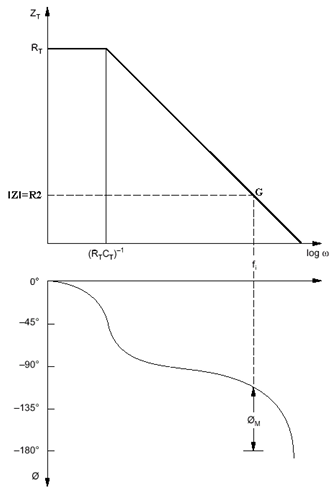
\includegraphics[width=0.5\linewidth]{Imagenes/5.12.png}
    \caption{}
    \label{fig:5.12}
\end{figure}
La expresión (\ref{eq:5.20}) y (\ref{eq:5.21}), permiten definir el método para la selección del valor de $R_2$, a partir de especificación del margen de fase. En efecto fijado este y siguiendo la línea de puntos en los diagramas de Fig 5.11, se determina el valor de la resistencia de realimentación, en el diagrama de módulo de la transimpedancia.

Para operar el dispositivo a frecuencias igual o inferior a la que correspondería un margen de fase de $90^\circ$, se puede considerar válida la expresión de la transimpedancia dada por (3.1) y aplicable el método expuesto para la selección de R2.

\begin{equation*}
    Z_T(s) = \frac{R_T}{1 + s \cdot C_T \cdot R_T}
\end{equation*}